\documentclass[a4paper, 12pt]{article}

\usepackage[left=2cm,right=2cm,
top=2cm,bottom=2cm,bindingoffset=0cm]{geometry}

\usepackage[T2A]{fontenc}
\usepackage[utf8]{inputenc}
\usepackage{color}
\usepackage{graphicx}
\usepackage{caption}
\usepackage{subcaption}
\usepackage{tikz}
\usepackage[english, russian]{babel}
\usepackage{ gensymb }
\usepackage{booktabs}
\usepackage{amsmath,amsfonts,amssymb,amsthm,mathtools}
\usepackage{lscape}
\usepackage{listings}

\begin{document}
\begin{center}
	\textbf{Метод конечных элементов для двумерной задачи упругости}

	\textbf{\textit{Задание}}
\end{center}

Дана прямоугольная пластина, левый край жестко защемлен, на правом действует равномерно распределенная нагрузка вдоль оси $X$ интенсивностью  $8\cdot 10^5 \text{Н/см}^2$. Толщина тела $t$ считается постоянной и равна 2 см. Модуль упругости  $E=2\cdot 10^7 \text{Н/см}^2$, коэффициент Пуассона $\mu=0.25$. Тело разбито на 8 треугольных элементов. Составить локальные матрицы жесткости и правых частей. Произвести сборку в глобальную матрицу и глобальный вектор. Решить СЛАУ.

\begin{figure}[h]
	\centering
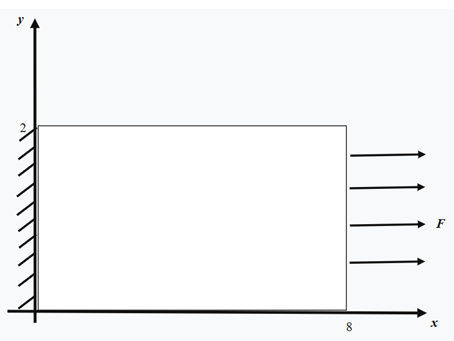
\includegraphics[width=0.5\linewidth]{zad.png}
\end{figure} 


\begin{center}
	\textit{\textbf{Решение}}
\end{center}

Рассмотрим задачу, соответствующую плоско-напряженному состоянию.  
Неизвестными функциями в данной задаче выступают перемещения \(u(x,y)\), \(v(x,y)\).  
Запишем неизвестные в векторном виде: \(u = \begin{bmatrix} u \\ v \end{bmatrix}\).

Неразмерность распределения перемещений будем определять антиградиентом, называемым деформациями 
\[
\varepsilon = \begin{bmatrix} \varepsilon_x \\ \varepsilon_y \\ \gamma_{xy} \end{bmatrix}^T
\]
где 
\[\varepsilon_x = \frac{\partial u}{\partial x}, \varepsilon_y = \frac{\partial v}{\partial y}, \gamma_{xy} = \frac{\partial u}{\partial y} + \frac{\partial v}{\partial x}
\]
или
\[
\varepsilon = L u, \quad L = 
\begin{bmatrix}
	\frac{\partial}{\partial x} & 0 \\
	0 & \frac{\partial}{\partial y} \\
	\frac{\partial}{\partial y} & \frac{\partial}{\partial x}
\end{bmatrix}.
\]

Деформации связаны с напряжением \(\sigma = \begin{bmatrix} \sigma_x \\ \sigma_y \\ \tau_{xy} \end{bmatrix}\) через физические соотношения (закон Гука): 
\[
\sigma = D \varepsilon = D L u
\]
где
\[
D = \frac{E}{1 - \mu^2}
\begin{bmatrix}
	1 & \mu & 0 \\
	\mu & 1 & 0 \\
	0 & 0 & \frac{1-\mu}{2}
\end{bmatrix}  \text{ — матрица упругости.}
\]

Составим вариационную постановку задачи.

Полная потенциальная энергия упругости системы равна \(\Pi = \Lambda - W_p\), где \(\Lambda\) — энергия деформаций, \(W_p\) — потенциальная энергия внешних сил.  
Энергия деформации задается формулой:
\[
\Lambda = \int\limits_V \frac{1}{2} \{\sigma^T \varepsilon\} \, dV,
\]
\[
W_p = \int\limits_S u^T p \, dS.
\]

Для решения задачи методом конечных элементов выразим перемещение через узловые значения \[
u = \left[N\right] \{\Phi\}
\]


Для треугольного симплекс элемента получаем:
\[
u = \begin{bmatrix} u \\ v \end{bmatrix} =
\begin{bmatrix}
	N_1 & 0 & N_2 & 0 & N_3 & 0 \\
	0 & N_1 & 0 & N_2 & 0 & N_3
\end{bmatrix}
\begin{bmatrix}
	u_1 \\ v_1 \\ u_2 \\ v_2 \\ u_3 \\ v_3
\end{bmatrix}.
\]
где \(N_1 = \frac{1}{2S^{(e)}}(a_i + b_i x + c_i y) = L_i, i = \overline{1,3}.\) Коэффициенты были выведены ранее:  
\[
a_1 = x_2 y_3 - x_3 y_2 \quad b_1 = y_2 - y_3 \quad c_1 = x_3 - x_2
\]
\[
a_2 = x_3 y_1 - x_1 y_3 \quad b_2 = y_3 - y_1 \quad c_2 = x_1 - x_3
\]
\[
a_3 = x_1 y_2 - x_2 y_1 \quad b_3 = y_1 - y_2 \quad c_3 = x_2 - x_1
\]

Тогда 
\[
\varepsilon = L u = LN \Phi = B \Phi
\]
\[
B^{(e)} = \frac{1}{2S(e)}
\begin{bmatrix}
	b_1 & 0 & b_2 & 0 & b_3 & 0 \\
	0 & c_1 & 0 & c_2 & 0 & c_3 \\
	c_1 & b_1 & c_2 & b_2 & c_3 & b_3
\end{bmatrix}.
\]

Внешние нагрузки в данном случае представляются в виде работы поверхностных сил:
\[
p = \begin{bmatrix} p_x \\ p_y \end{bmatrix}, \quad W_p =\int\limits_S \Phi^T N^T \begin{bmatrix} p_x \\ p_y \end{bmatrix} dS.
\]

Все полученные формулы подставим в формулу полной энергии (для симплекс элемента):
\[
\Pi^{(e)} = \frac{1}{2} \int\limits_{V^{(e)}} \Phi^{(e)T} B^{(e)T} D B^{(e)} \Phi^{(e)} dV - \int\limits_S \Phi^{(e)T} N^{(e)T} \begin{bmatrix} p_x^{(e)} \\ p_y^{(e)} \end{bmatrix} \, dS.
\]

Для минимизации функционала \(\Pi\) найдем производную и приравняем её к нулю:
\[
\frac{\partial \Pi^{(e)}}{\partial \Phi^{i}} = \int\limits_{V^{(e)}} B^{(e)T} D^{(e)} B^{(e)} \Phi^{(e)} \, dV - \int\limits_S N^{(e)T} \begin{bmatrix} p_x^{(e)} \\ p_y^{(e)} \end{bmatrix} \, dS = 0.
\]


\[
K^{(e)} = \int\limits_{V^{(e)}} B^{(e)T} D^{(e)} B^{(e)} \, dV, \quad f^{(e)} = \int\limits_{S} N^{(e)T} \begin{bmatrix} p_x^{(e)} \\ p_y^{(e)} \end{bmatrix} \, dS
\]

Следовательно, можно представить в виде СЛАУ:
\[
K^{(e)} \Phi = f^{(e)}.
\]

Выразим матрицу \(K^{(e)}\) и вектор правой части \(f^{(e)}\) через специальные формулы:
\[
\int\limits_{S(e)} L_1^{\alpha} L_2^{\beta} L_3^{\gamma} \, dS = \frac{\alpha! \, \beta! \, \gamma!}{(\alpha + \beta + \gamma + 2)!} 2S(e), \quad
\int\limits_{\Gamma_{12}^{(e)}} L_1^{\alpha} L_2^{\beta} \, d\Gamma = \frac{\alpha! \, \beta!}{(\alpha + \beta + 1)!} l_{ij}.
\]

Так как толщины пластины постоянна,  \(dV = t \, dS\). Тогда:
\[
K^{(e)} = t \int\limits_{S^{(e)}} B^{(e)T} D^{(e)} B^{(e)} \, dS =t \, B^{(e)T} D^{(e)} B^{(e)} S^{(e)}.
\]

Для граничных узлов можно выразить \(dS = t \, d\Gamma\), причем учитываться будут только \(\Gamma_{ij}\), где \(i,j\) — граничные, причем \(p_y^{(e)} = 0\), так как нагрузка действует только вдоль оси \(Ox\), а также \(N_k = 0\), так как нагрузка приходится только на два узла \(i,j\):
\[
f^{(e)} = t \int\limits_{\Gamma_{ij}^{(e)}} \begin{bmatrix}
	N_1 & 0 \\ 0 & N_1 \\
	N_2 & 0 \\ 0 & N_2 \\
	0 & 0 \\ 0 & 0 
\end{bmatrix}
\begin{bmatrix}
	p_x^{(e)} \\ 0
\end{bmatrix}
\, d\Gamma = t \int\limits_{\Gamma_{ij}^{(e)}}
\begin{bmatrix}
	L_1 & 0 \\ 0 & L_1 \\
	L_2 & 0 \\ 0 & L_2 \\
	0 & 0 \\ 0 & 0 
\end{bmatrix}
\begin{bmatrix}
	p_x^{(e)} \\ 0
\end{bmatrix} \, d\Gamma= \frac{tl_{ij}}{2}
\begin{bmatrix}
	1 & 0 \\ 0 & 1 \\
	1 & 0 \\ 0 & 1 \\
	0 & 0 \\ 0 & 0 
\end{bmatrix} \begin{bmatrix}
p_x^{(e)} \\ 0
\end{bmatrix} = \frac{tl_{ij} p_x^{(e)}}{2} \begin{bmatrix}
1\\0\\1\\0\\0\\0
\end{bmatrix}
\]

Дискретизация области:
\begin{figure}[h]
	\centering
	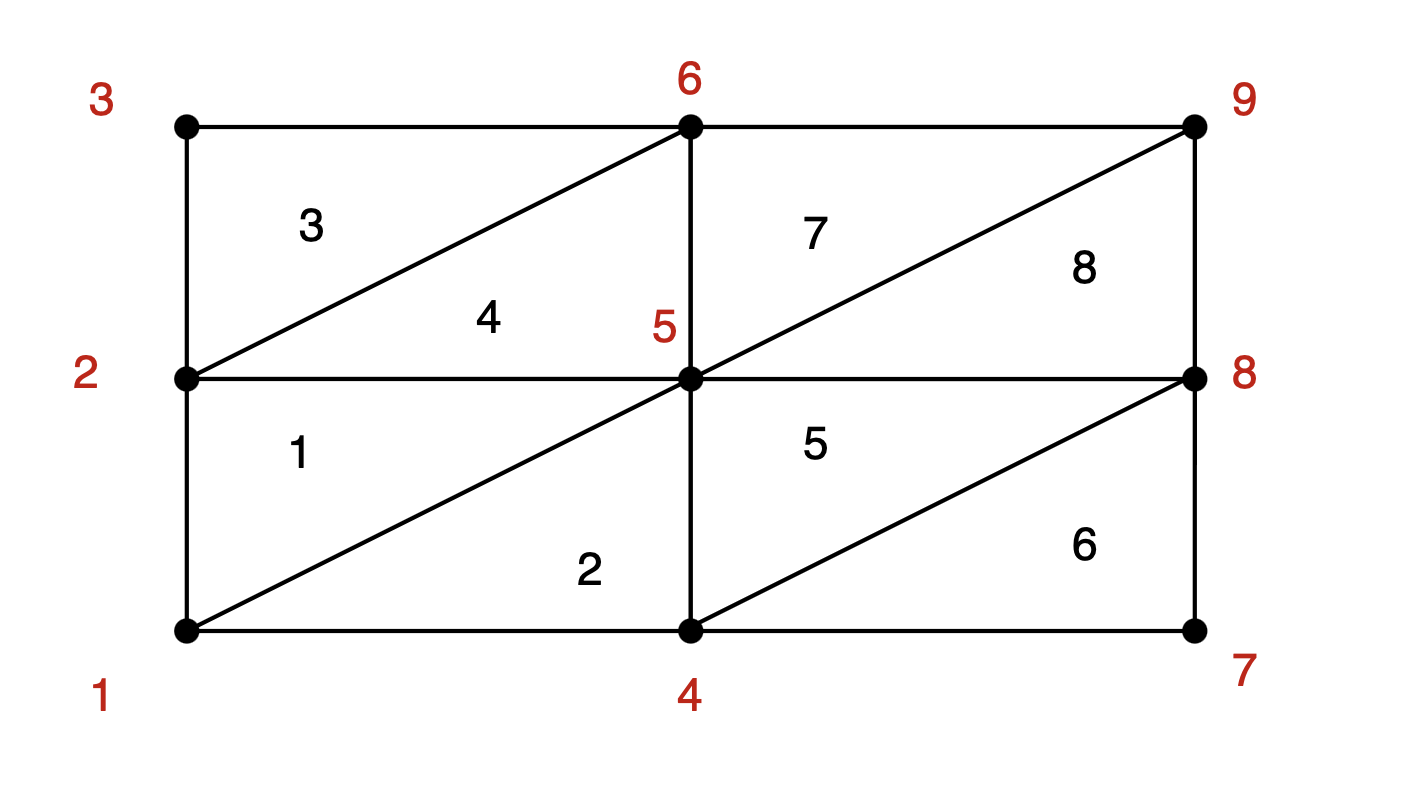
\includegraphics[width=0.5\linewidth]{treygolnichki.png}
\end{figure} 

\end{document}